% !TEX TS-program = pdflatexmk

\documentclass[14pt]{beamer}
\usepackage{newtxtext,newtxmath}
\usepackage{microtype}
\usepackage[english]{babel}
\usepackage{hyperref}
\usepackage{graphicx}
\usepackage{listings}
\lstloadlanguages{Python}
\lstset{language=Python}
\lstset{%
basicstyle=\ttfamily\bfseries,
keywordstyle=\color{blue}, emph={self}, emphstyle={\color{blue}},
identifierstyle=,
commentstyle=\color{brown},
stringstyle=\color{green!50!black},
showstringspaces=false,
emphstyle={[2]\color{purple}},
}
\usepackage{tikz}
\usepackage{forest}
\usetikzlibrary{positioning}
\usepackage{array}
\newcolumntype{L}[1]{>{\raggedright\let\newline\\\arraybackslash\hspace{0pt}}m{#1}}

\mode<presentation>{
\usetheme{Madrid}
\definecolor{uabgreen}{cmyk}{.89,.31,.78,.17}
\usecolortheme[named=uabgreen]{structure}
\setbeamertemplate{navigation symbols}{}
\setbeamertemplate{footline}[frame number]
\setbeamertemplate{section in toc}[square]
\setbeamertemplate{subsection in toc}[square]
\setbeamertemplate{items}[square]
\setbeamercovered{transparent=5}
}

\newcommand{\keyword}[1]{{\color{blue}#1}}
\newcommand{\cmnt}[1]{{\color{gray}#1}}
\newcommand{\str}[1]{{\color{green!50!black}#1}}
\newcommand{\defn}[1]{{\color{purple}#1}}

\author[Dr. Bethard]{Dr. Steven Bethard}
\institute[UAB CIS]{%
Computer and Information Sciences\\
University of Alabama at Birmingham}

\AtBeginSection[]
{
  \begin{frame}<beamer>{Outline}
    \tableofcontents[currentsection]
  \end{frame}
}

\tikzset{
  invisible/.style={opacity=0,text opacity=0},
  visible on/.code={%
    \alt<#1>{}{\pgfkeysalso{invisible}}
  },
  filled on/.code={%
    \alt<#1>{\pgfkeysalso{fill=gray}}{}
  },
}
\forestset{
  edge weight/.style={
    edge label={node[midway,above,sloped]{#1}}},
  invisible/.style={
    /tikz/invisible,
    edge={/tikz/invisible}},
  visible on filled on/.code n args={2}{%
    \alt<#1>{\alt<#2>{\pgfkeysalso{fill=gray}}{}}{\pgfkeysalso{invisible}}
  },
  visible on/.code={%
    \alt<#1>{}{\pgfkeysalso{invisible}}
  },
}

\lstset{emph={[2]__init__,__str__}}

\title{Adversarial Search}
\date[]{16 Jan 2014}

\newcommand{\tictactoe}[9]{
\begin{tabular}{@{} c @{\hspace{0.2em}} | @{\hspace{0.2em}} c @{\hspace{0.2em}} | @{\hspace{0.2em}} c @{\hspace{0.2em}}}
#1 & #2 & #3 \\
\hline
#4 & #5 & #6 \\
\hline
#7 & #8 & #9 \\
\end{tabular}
}
\newcommand{\abcutil}[3]{(#1,#2,#3)}
\newcommand{\utilab}[3]{%
#1{\tiny
\begin{tabular}{ l @{} >{\centering\arraybackslash}m{2.2em} @{}}
$\geq$ & $#2$ \\
$\leq$ & $#3$
\end{tabular}}}

\begin{document}

\begin{frame}
  \titlepage
\end{frame}

\begin{frame}{Outline}
  \tableofcontents
\end{frame}

\section{Describing Games}
\subsection{Games as Search}
\begin{frame}{Games as Search}
	\begin{block}{Games as Search}
		\begin{description}
			\item[Initial] A board position and which player is to move
			\item[Actions] Moves and resulting states
			\item[Goal] A terminal state, where the game has ended
			\item[Score] Based on utility function, e.g. +1 win, -1 lose
		\end{description}
	\end{block}
	\pause
	\begin{block}{Game Types}
		\centering
		\hyphenpenalty=10000
		\begin{tabular}{ L{0.2\textwidth} | L{0.3\textwidth} | L{0.3\textwidth}}
			                    & Deterministic               & Stochastic \\
			\hline
			Perfect information       & \uncover<3->{chess, checkers, go, reversi}     & \uncover<4->{backgammon, monopoly} \\
			\hline
			Imperfect information    & \uncover<5->{battleship, blind tic-tac-toe}          & \uncover<6->{bridge, poker, scrabble} \\
		\end{tabular}
	\end{block}
\end{frame}
\subsection{Game Search Trees}
\begin{frame}{Tic-Tac-Toe Game Tree}
	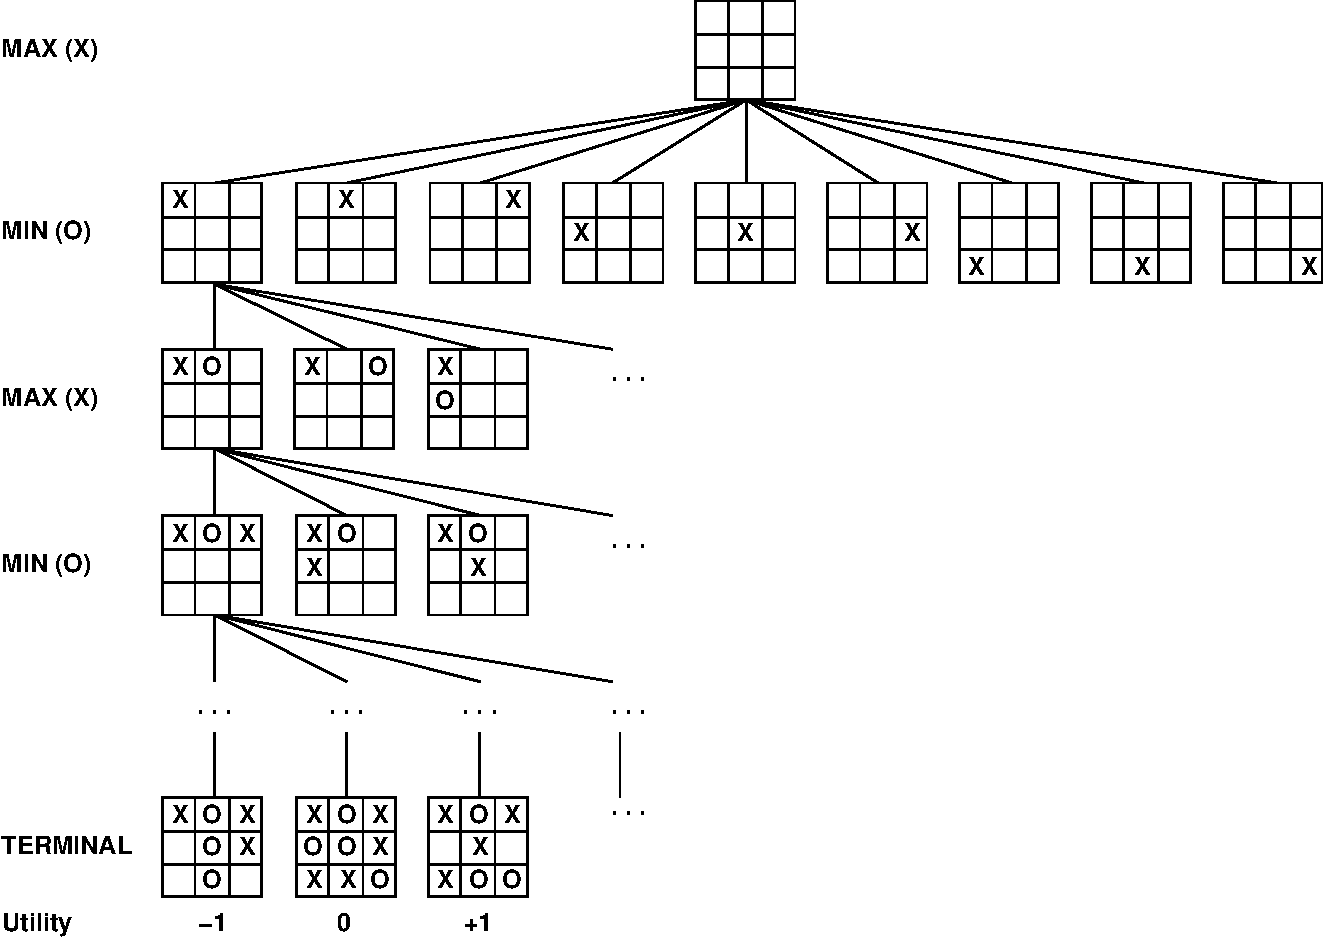
\includegraphics[width=4in]{tictactoe.pdf}
\end{frame}

\section{Deterministic Games}
\subsection{Minimax}
\begin{frame}[fragile,label=minimax-example]{Minimax}
\begin{block}{Idea}
\begin{itemize}
\item Expect other player to minimize your utility
\item Choose action that maximizes the minimized utility
\end{itemize}
\end{block}
\begin{center}
\small
\begin{forest}
left action/.style={
  edge label={node[midway,left]{\small #1}}},
middle action/.style={
  edge label={node[midway,left=-0.25em]{\small #1}}},
right action/.style={
  edge label={node[midway,right]{\small #1}}},
for tree={minimum size=1.5em,l sep=3em,s sep=1.2em}
[{},phantom
  [{Max Player},edge=invisible
    [{Min Player},edge=invisible
      [{Max Player},invisible]
    ]
  ]
  [{3},edge=invisible,for tree={draw},text visible on={11}
    [{3},left action={$a_1$},visible on={2-10},text visible on={4-10}
      [{3},left action={$b_1$},visible on={3}]
      [{12},middle action={$b_2$},visible on={3}]
      [{8},right action={$b_3$},visible on={3}]
    ]
    [{2},middle action={$a_2$},visible on={5-10},text visible on={7-10}
      [{2},left action={$c_1$},visible on={6}] 
      [{4},middle action={$c_2$},visible on={6}]
      [{6},right action={$c_3$},visible on={6}]
    ]
    [{2},right action={$a_3$},visible on={8-10},text visible on={10-10}
      [{14},left action={$d_1$},visible on={9}]
      [{5},middle action={$d_2$},visible on={9}]
      [{2},right action={$d_3$},visible on={9}]
    ]
  ]
]
\end{forest}
\end{center}
\end{frame}
\begin{frame}[fragile]{Minimax Code}
	\begin{semiverbatim}\scriptsize\bfseries
		\keyword{def} \defn{minimax_decision}(problem, state):
		    \pause\cmnt{# select the action with the maximum utility}
		    action, utility = select_action(max, problem, state)
		    \keyword{return} action
		\pause
		\keyword{def} \defn{select_action}(get_best, problem, state):
		    \pause\cmnt{# for leaf nodes, just return the known utility}
		    \keyword{if} problem.is_terminal(state):
		        \keyword{return} \keyword{None}, problem.get_utility(state)
		    \pause\cmnt{# otherwise, recursively collect utility values for available actions}
		    items = []
		    \keyword{for} action, state \keyword{in} problem.get_successors(state):
		        get_worst = min \keyword{if} get_best == max \keyword{else} max
		        _, utility = select_action(get_worst, problem, state)
		        items.append((action, utility))
		    \pause\cmnt{# return the action with the best utility}
		    \keyword{return} get_best(items)
	\end{semiverbatim}
\end{frame}
\begin{frame}{Minimax Exercise}
	\begin{columns}
		\begin{column}{2in}
			\begin{block}{Build Minimax Tree}
				\begin{itemize}
					\item It is X's turn
					\item Scoring: \\
						\begin{tabular}{lr}
							X Wins      & +1 \\
							X Loses     & -1 \\
							X and O Tie &  0 \\
						\end{tabular}
				\end{itemize}
			\end{block}
		\end{column}
		\begin{column}{2in}
			\centering
			\Huge
			\tictactoe{O}{X}{X}{X}{ }{ }{O}{O}{ }
		\end{column}
	\end{columns}
\end{frame}
\begin{frame}{Minimax Exercise}
\begin{center}
\scriptsize
\begin{forest}
for tree={align=center,s sep=2em}
[{\tictactoe{O}{X}{X}{X}{ }{ }{O}{O}{ } \\ $f(n) = 0$}
  [{\tictactoe{O}{X}{X}{X}{X}{ }{O}{O}{ } \\ $f(n) = -1$}
    [{\tictactoe{O}{X}{X}{X}{X}{O}{O}{O}{ } \\ $f(n) = 0$}
      [{\tictactoe{O}{X}{X}{X}{X}{O}{O}{O}{X} \\ $f(n) = 0$}]
    ]
    [{\tictactoe{O}{X}{X}{X}{X}{ }{O}{O}{O} \\ $f(n) = -1$}]
  ]
  [{\tictactoe{O}{X}{X}{X}{ }{X}{O}{O}{ } \\ $f(n) = -1$}
    [{\tictactoe{O}{X}{X}{X}{O}{X}{O}{O}{ } \\ $f(n) = +1$}
      [{\tictactoe{O}{X}{X}{X}{O}{X}{O}{O}{X} \\ $f(n) = +1$}]
    ]
    [{\tictactoe{O}{X}{X}{X}{ }{X}{O}{O}{O} \\ $f(n) = -1$}]
  ]
  [{\tictactoe{O}{X}{X}{X}{ }{ }{O}{O}{X} \\ $f(n) = 0$}
    [{\tictactoe{O}{X}{X}{X}{O}{ }{O}{O}{X} \\ $f(n) = +1$}
      [{\tictactoe{O}{X}{X}{X}{O}{X}{O}{O}{X} \\ $f(n) = +1$}]
    ]
    [{\tictactoe{O}{X}{X}{X}{ }{O}{O}{O}{X} \\ $f(n) = 0$}
      [{\tictactoe{O}{X}{X}{X}{X}{O}{O}{O}{X} \\ $f(n) = 0$}]
    ]
  ]
]
\end{forest}
\end{center}
\end{frame}
\begin{frame}[fragile,label=minimax-properties]{Minimax Properties}
\begin{center}
\small
\begin{forest}
left action/.style={
  edge label={node[midway,left]{\small #1}}},
middle action/.style={
  edge label={node[midway,left=-0.25em]{\small #1}}},
right action/.style={
  edge label={node[midway,right]{\small #1}}},
for tree={minimum size=1.5em,l sep=3em,s sep=1.2em}
[{},phantom
  [{Max Player},edge=invisible
    [{Min Player},edge=invisible
      [{Max Player},invisible]
    ]
  ]
  [{3},edge=invisible,for tree={draw},text opacity=0
    [{3},left action={$a_1$},for children=invisible
      [{3},left action={$b_1$}]
      [{12},middle action={$b_2$}]
      [{8},right action={$b_3$}]
    ]
    [{2},middle action={$a_2$},text opacity=0
      [{2},left action={$c_1$}] 
      [{4},middle action={$c_2$}]
      [{6},right action={$c_3$}]
    ]
    [{2},right action={$a_3$},text opacity=0,for children=invisible
      [{14},left action={$d_1$}]
      [{5},middle action={$d_2$}]
      [{2},right action={$d_3$}]
    ]
  ]
]
\end{forest}
\end{center}
\begin{tabular}{ll}
Complete? & \uncover<2->{Yes, if tree is finite} \\
Optimal?   & \uncover<3->{Yes, for optimal opponent} \\
Time? & \uncover<4->{$O(b^m)$, all nodes in the tree} \\
Space? & \uncover<5->{$O(bm)$, like depth first search} \\
\end{tabular}
\end{frame}
\begin{frame}{Multiplayer Minimax}
\begin{center}
\scriptsize
\begin{forest}
for tree={align=center,minimum size=1.5em,l sep=3em,s sep=1.25em}
[{},phantom
  [{Player 0},edge=invisible
    [{Player 1},edge=invisible
      [{Player 2},edge=invisible
        [{Player 0},edge=invisible]
      ]
    ]
  ]
  [{\abcutil{1}{2}{6}},for tree={draw},text visible on={8-}
    [{\abcutil{1}{2}{6}},text visible on={4-}
      [{\abcutil{1}{2}{6}},text visible on={2-}
        [{\abcutil{1}{2}{6}}
          [{\ldots},draw=none]
        ]
        [{\abcutil{4}{2}{3}}
          [{\ldots},draw=none]
        ]
      ]
      [{\abcutil{6}{1}{2}},text visible on={3-}
        [{\abcutil{6}{1}{2}}
          [{\ldots},draw=none]
        ]
        [{\abcutil{7}{4}{1}}
          [{\ldots},draw=none]
        ]
      ]
    ]
    [{\abcutil{1}{5}{2}},text visible on={7-}
      [{\abcutil{1}{5}{2}},text visible on={5-}
        [{\abcutil{5}{1}{1}}
          [{\ldots},draw=none]
        ]
        [{\abcutil{1}{5}{2}}
          [{\ldots},draw=none]
        ]
      ]
      [{\abcutil{5}{4}{5}},text visible on={6-}
        [{\abcutil{7}{7}{1}}
          [{\ldots},draw=none]
        ]
        [{\abcutil{5}{4}{5}}
          [{\ldots},draw=none]
        ]
      ]
    ]
  ]
]
\end{forest}
\end{center}
\end{frame}

\subsection{Alpha-Beta Pruning}
\begin{frame}[label=alpha-beta-pruning-example]{Alpha-Beta Pruning}
% from http://www.cs.ucla.edu/~rosen/161/notes/alphabeta.html
\begin{center}
\footnotesize
\begin{forest}
pruned/.style={draw=none,content={---}}
[{},phantom,for tree={align=center}
  [{Max},for tree={edge=invisible,l sep*=1.25}
    [{Min}
      [{Max}
	[{Min}
	  [{Max},invisible]
	]
      ]
    ]
  ]
  [{\utilab{\visible<41->{3}}{\alt<25->{3}{-\infty}}{+\infty}},for tree={draw}
    [{\utilab{\visible<24->{3}}{-\infty}{\alt<16->{3}{+\infty}}},visible on={2-40}
      [{\utilab{\visible<15->{3}}{\alt<9->{3}{-\infty}}{+\infty}},visible on={3-23}
        [{\utilab{\visible<8->{3}}{-\infty}{\alt<6->{3}{+\infty}}},visible on={4-14}
          [{3},visible on={5-7}]
          [{17},visible on={7}]
        ]
        [{\utilab{\visible<14->{2}}{3}{\alt<12->{2}{+\infty}}},visible on={10-14}
          [{2},visible on={11-13}]
          [{12},pruned,visible on={13}]
        ]
      ]
      [{\utilab{\visible<23->{15}}{\alt<21->{15}{-\infty}}{3}},visible on={17-23}
        [{\utilab{\visible<20->{15}}{-\infty}{3}},visible on={18-22}
          [{15},visible on={19}]
        ]
        [{},pruned,visible on={22}
          [{25},invisible]
          [{0},invisible]
        ]
      ]
    ]
    [{\utilab{\visible<40->{3}}{3}{\alt<38->{3}{+\infty}}},visible on={26-40}
      [{\utilab{\visible<37->{3}}{3}{+\infty}},visible on={27-39}
        [{\utilab{\visible<32->{2}}{3}{\alt<30->{2}{+\infty}}}, visible on={28-36}
          [{2},visible on={29-31}]
          [{5},pruned,visible on={31}]
        ]
        [{\utilab{\visible<36->{3}}{3}{\alt<35->{3}{+\infty}}},visible on={33-36}
          [{3},visible on={34-35}]
        ]
      ]
      [{},pruned,visible on={39}
        [{},invisible
          [{2},invisible]
          [{14},invisible]
        ]
      ]
    ]
  ]
]
\end{forest}
\end{center}
\end{frame}
\begin{frame}{Alpha-Beta Pruning in General}
	\begin{columns}
		\begin{column}{2in}
			\begin{block}{Idea}
				If $m$ is a better choice, then $n$ will never be reached
			\end{block}
			\begin{block}<2->{Alpha-Beta Bookkeeping}
				\begin{itemize}
					\item[$\alpha$] Best value for Player \\ (the highest value)
					\item[$\beta$] Best value for Opp \\ (the lowest value)
				\end{itemize}
			\end{block}
		\end{column}
		\begin{column}{2in}
			\begin{center}
				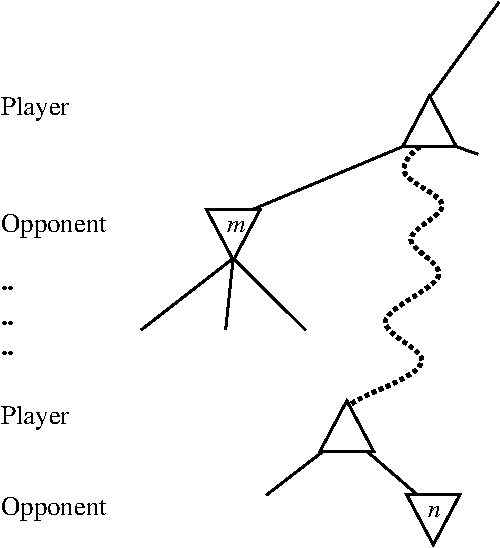
\includegraphics[width=2in]{alpha-beta-general.pdf}
			\end{center}
		\end{column}
	\end{columns}
\end{frame}
\begin{frame}[fragile]{Alpha-Beta Pruning Code}
	\begin{semiverbatim}\scriptsize\bfseries
		\keyword{def} \defn{alpha_beta_search}(problem, state):
		    \pause\cmnt{# select the action with the maximum utility}
		    value, action = max_ab(state, neg_inf, pos_inf)
		    \keyword{return} action
		\pause
		\keyword{def} \defn{\alt<9>{\alert{min}}{max}_ab}(problem, state, alpha, beta):
		    \pause\cmnt{# simply return the known utility for leaf nodes}
		    \keyword{if} problem.is_terminal(state):
		        \keyword{return} problem.get_utility(state), \keyword{None}
		    \pause\cmnt{# examine utility values for each available action}
		    value, action = neg_inf, \keyword{None}
		    \keyword{for} action2, state2 \keyword{in} problem.get_successors(state):
		        value2, _ = \alt<9>{\alert{max}}{min}_ab(problem, state2, alpha, beta)
		        \pause\cmnt{# return the new value if \alt<9>{\alert{lower }}{higher} than the global \alt<9>{\alert{max}}{min}imum}
		        value, action = \alt<9>{\alert{min}}{max}([value, action], [value2, action2])
		        \keyword{if} value\alt<9>{\alert{ <= alpha}}{ >=  beta}:
		            \keyword{return} value, action
		        \pause\cmnt{# otherwise, update the global \alt<9>{\alert{min}}{max}imum}
		        \alt<9>{\alert{beta }}{alpha} = \alt<9>{\alert{min}}{max}(\alt<9>{\alert{beta}, }{alpha,} value)
		    \pause\cmnt{# return the action with the \alt<9>{\alert{min}}{max}imum utility}
		    \keyword{return} value, action
	\end{semiverbatim}
\end{frame}
\begin{frame}[label=alpha-beta-pruning-properties]{Alpha-Beta Pruning Properties}
\begin{center}
\footnotesize
\begin{forest}
pruned/.style={draw=none,content={---}}
[{},phantom,for tree={align=center}
  [{Max},for tree={edge=invisible,l sep*=1.25}
    [{Min}
      [{Max}
	[{Min}]
      ]
    ]
  ]
  [{\utilab{\invisible{3}}{-\infty}{+\infty}},for tree={draw}
    [{\utilab{\invisible{3}}{-\infty}{3}}
      [{\utilab{3}{3}{+\infty}}
        [{\utilab{3}{-\infty}{3}},invisible]
        [{\utilab{2}{3}{2}},invisible]
      ]
      [{\utilab{\invisible{15}}{15}{3}}
        [{\utilab{15}{-\infty}{3}}]
        [{},pruned]
      ]
    ]
    [{\utilab{3}{3}{+\infty}},invisible
      [{\utilab{3}{3}{+\infty}},invisible]
      [{},pruned,invisible]
    ]
  ]
]
\end{forest}
\end{center}
	\begin{block}{Time Complexity}
		\begin{itemize}
			\pause
			\item ``Perfectly'' ordered branches gives $O(b^{m/2})$
			\pause
			\item Still exponential, but doubles solvable depth
		\end{itemize}
	\end{block}
\end{frame}

\subsection{Approximate Solutions}
\begin{frame}[fragile]{Approximate Solutions}
	\begin{block}{Problem}
		Even with Alpha-Beta Pruning, chess space is still $35^{50}$
	\end{block}
	\pause
	\begin{block}{Solution}
		Don't search the entire tree:
		\begin{semiverbatim}\scriptsize\bfseries
		    \keyword{if} problem.\alt<3->{\alert{is_past_cutoff}}{is_terminal}(state):
		        \keyword{return} problem.\alt<3->{\alert{get_estimated_utility}}{get_utility}(state)
		
		\end{semiverbatim}
	\end{block}
	\pause\pause
	\begin{block}{Example}
		\begin{itemize}
			\item Given 100 seconds
			\item Given ability to explore $10^4$ nodes/second
			\item Can explore to depth $\approx 8$ ($10^6 \approx 35^{8/2}$)
		\end{itemize}
	\end{block}
\end{frame}
\begin{frame}{Evaluation Functions}
	\begin{block}{Necessary Properties}
		\begin{itemize}
			\item Quickly computable
			\item Orders terminal states by utility
			\item Correlated with chances of winning
		\end{itemize}
	\end{block}
	\pause
	\begin{block}{Typical Approach}
		Weighted linear combination of features:
		\[\mbox{\sc Eval}(s) = w_1 f_1(s) + w_1 f_2(s) + \ldots + w_n f_n(s)\]
	\end{block}
\end{frame}
\begin{frame}{Example Evaluation Function}
	\centering
	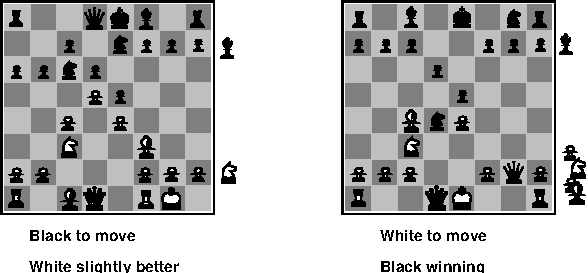
\includegraphics[height=1.75in]{chess-evaluation.pdf}
	\begin{block}{Weighted Features}
		\small
		$
		\begin{array}{rcl}
			w_{\mbox{\scriptsize pawn}}  \cdot f_{\mbox{\scriptsize pawn}}(s)  & = & 1 \cdot (\mbox{white pawns} - \mbox{black pawns})   \\
			\ldots                                                             & = & \ldots \\
			w_{\mbox{\scriptsize queen}} \cdot f_{\mbox{\scriptsize queen}}(s) & = & 9 \cdot (\mbox{white queens} - \mbox{black queens})
		\end{array}
		$
	\end{block}
\end{frame}
\begin{frame}{Deterministic Games in Practice}
	\begin{block}{Checkers}
		\begin{itemize}
			\item\small 1994: Chinook ``Man-Machine World Champion'' (0-0-6)
			\item\small 2007: Chinook's creators ``proved'' it cannot lose
			\item\small End-game database for all $\leq 10$ piece states
		\end{itemize}
	\end{block}
	\begin{block}{Chess}
		\begin{itemize}
			\item\small 1997: Deep Blue defeated Garry Kasparov (2-1-3)
			\item\small 200 million positions per second, searching 6-40 plies
			\item\small End-game database for all $\leq 5$ piece states
		\end{itemize}
	\end{block}
	\begin{block}{Go}
		\begin{itemize}
			\item\small Computers still rank as intermediate amateurs
			\item\small Go has $\approx 150$�-$250$ moves per turn
		\end{itemize}
	\end{block}
\end{frame}

\section{Nondeterministic Games}

\subsection{Describing Nondeterministic Games}
\begin{frame}{Nondeterministic Game: Backgammon}
	\begin{center}
		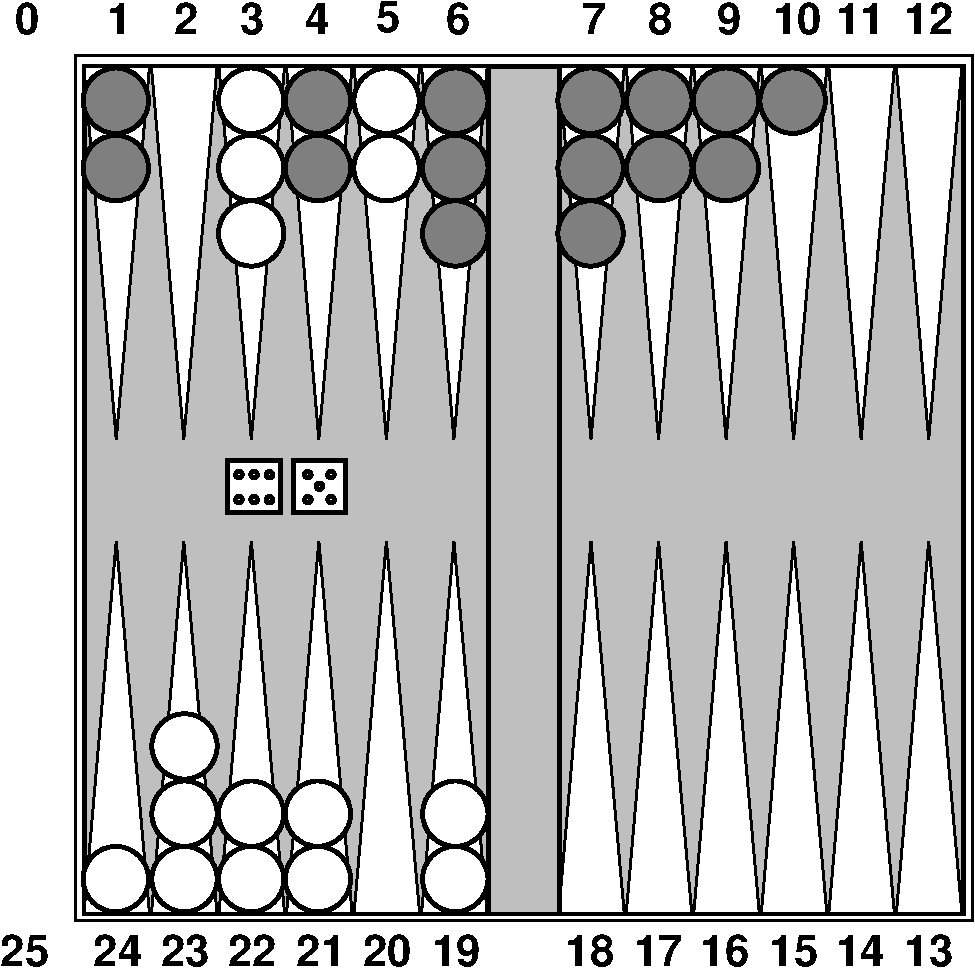
\includegraphics[height=2.5in]{backgammon-position.pdf}
	\end{center}
\end{frame}
\begin{frame}{Backgammon Game Tree}
	\begin{center}
		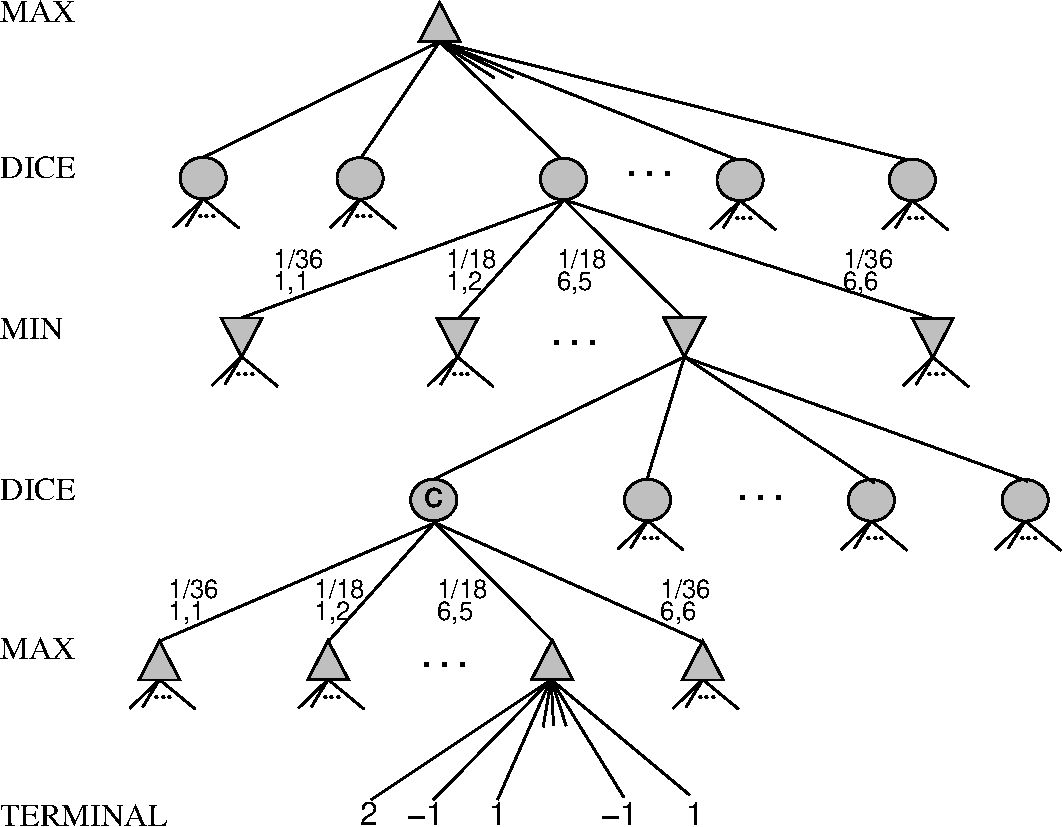
\includegraphics[height=2.5in]{backgammon-tree.pdf}
	\end{center}
\end{frame}

\subsection{Expectiminimax}
\begin{frame}{Expectiminimax}
	\begin{block}{Expected Values for Chance Nodes}
		\[\textsc{Expecti}(n) = \sum\limits_{s \in \textsc{\scriptsize Successors}(n)}{P(s) \cdot \textsc{Expecti}(s)}\]
	\end{block}
	\begin{center}
		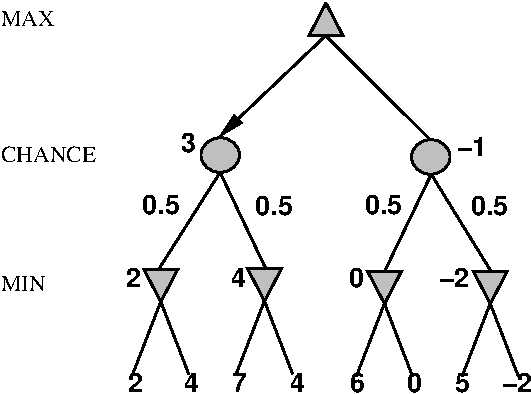
\includegraphics[height=1.75in]{expectiminimax-simple.pdf}
	\end{center}
\end{frame}
\begin{frame}{Expectiminimax Practice}
	\begin{block}{A Simple Game}
		\begin{itemize}
			\item Deck contains J, Q, K, K
			\item One card will be selected by the players
			\item Player 1 draws first, and either:
				\begin{itemize}
					\item Keeps the card and the game is over, or
					\item Removes the card and Player 2 draws and either:
						\begin{itemize}
							\item Keeps the card and the game is over
							\item Discards the card and a final card is drawn
						\end{itemize}
				\end{itemize}
			\item A final J scores -1, Q scores 0, and K scores +1
		\end{itemize}
	\end{block}
\end{frame}
\begin{frame}{Using Expectiminimax}
	\begin{block}{Expectiminimax Properties}
		\begin{tabular}{ll}
			Complete? \pause & Yes, if tree is finite (both moves and ``rolls'') \pause \\
			Optimal?  \pause & Yes \pause \\
			Time?     \pause & $O(b^mn^m)$, all nodes, all ``roll'' sequences \\
		\end{tabular}
	\end{block}
	\pause
	\begin{block}{Consequences}
		\begin{tabular}{ll}
			Branching Factor?   \pause & Increased by dice rolls \pause \\
			Node Likelihood?    \pause & Decreases with depth \pause \\
			Alpha-Beta Pruning? \pause & Effectiveness decreased \\
		\end{tabular}
	\end{block}
	\pause
	\begin{block}{Real-World Example: TD-Gammon}
		\begin{itemize}
			\item Depth-2 search, no Alpha-Beta pruning
			\item Neural network eval function trained by self-play
		\end{itemize}
	\end{block}
\end{frame}
\begin{frame}{Utilities in Expectiminimax}
	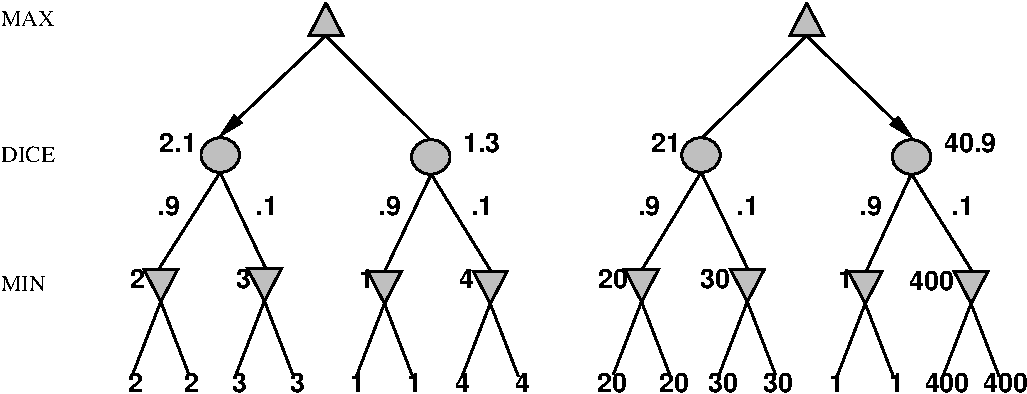
\includegraphics[width=4in]{utility-chance.pdf}
	\pause
	\\ \bigskip
	\begin{block}{Requirement}
		Evaluation function must be a linear transform of utility
	\end{block}
\end{frame}
\begin{frame}{Utilities in Deterministic Games}
	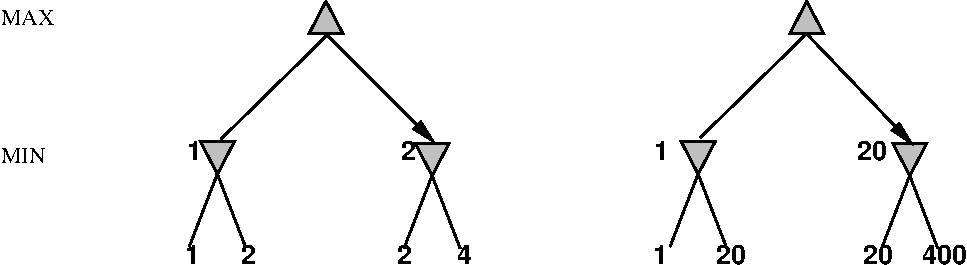
\includegraphics[width=4in]{utility-deterministic.pdf}
	\pause
	\\ \bigskip
	\begin{block}{Requirement}
		Evaluation function need only match the utility ordering
	\end{block}
\end{frame}

\subsection{Games with Imperfect Information}
\begin{frame}[t]{Imperfect Information: Bridge}
	\bigskip
	\only<1>{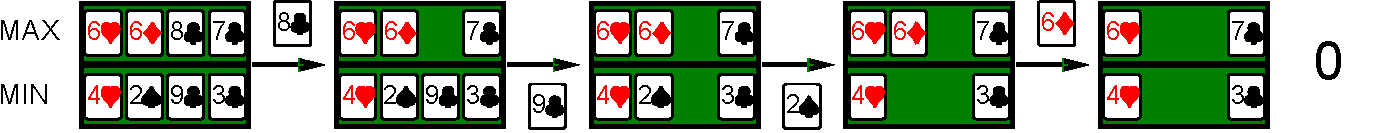
\includegraphics[width=4.2in]{card-tree-1.pdf}}%
	\only<2>{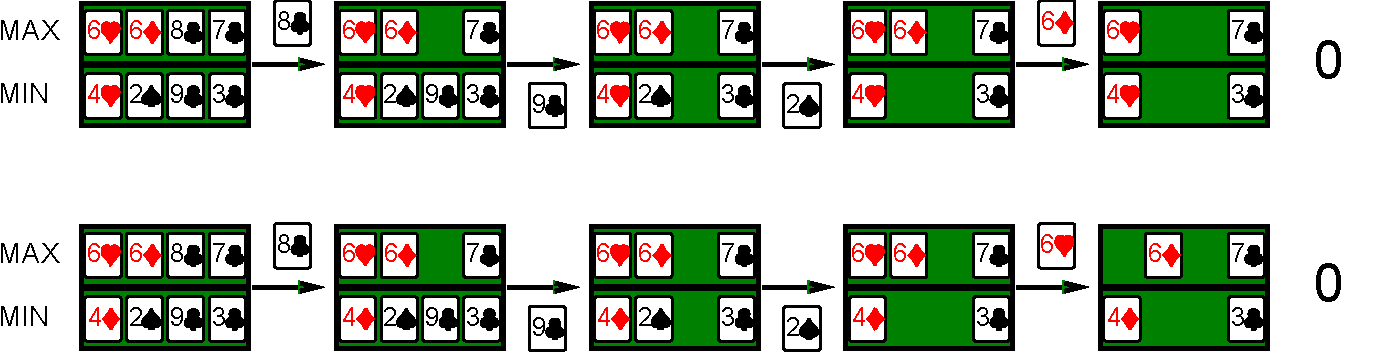
\includegraphics[width=4.2in]{card-tree-2.pdf}}%
	\only<3>{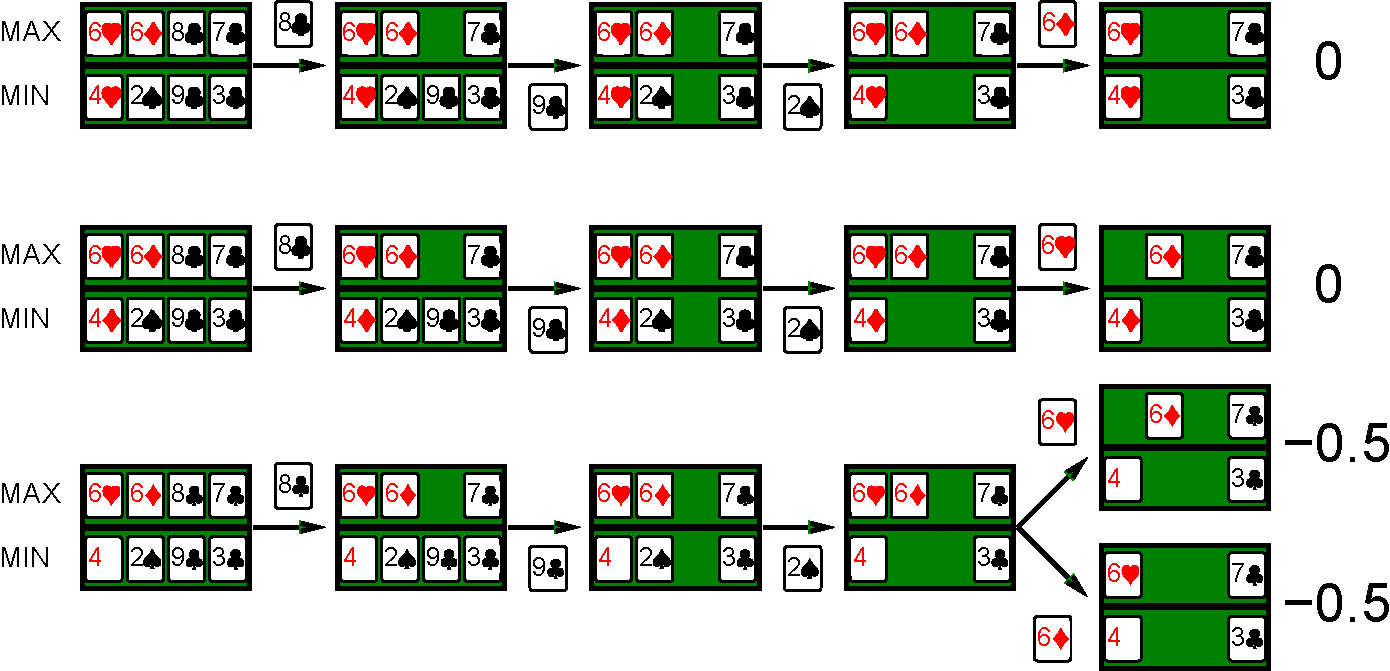
\includegraphics[width=4.2in]{card-tree-3.pdf}}%
\end{frame}
\begin{frame}{Imperfect Information: Common Sense}
	\begin{itemize}
		\item Road A leads to a small heap of gold pieces
		\item \alert<2->{Road B} leads to a fork:
			\begin{itemize}
				\item Take the \alert<2->{left fork} and you'll find a mound of jewels
				\item Take the right fork and you'll be run over by a bus
			\end{itemize}
	\end{itemize}
	\begin{itemize}
		\item<3-> Road A leads to a small heap of gold pieces
		\item<3-> \alert<4->{Road B} leads to a fork:
			\begin{itemize}
				\item<3-> Take the left fork and you'll be run over by a bus
				\item<3-> Take the \alert<4->{right fork} and you'll find a mound of jewels
			\end{itemize}
	\end{itemize}
	\begin{itemize}
		\item<5-> \alert<6->{Road A} leads to a small heap of gold pieces
		\item<5-> Road B leads to a fork:
			\begin{itemize}
				\item<5-> Guess correctly and you'll find a mound of jewels
				\item<5-> Guess incorrectly and you'll be run over by a bus
			\end{itemize}
	\end{itemize}
\end{frame}
\begin{frame}{Imperfect Information}
	\begin{block}{Key Point}
		Value of an action \alert{is not} the average across all states \\
		\pause
		Should be searching through a tree of \alert{belief} states, and:
		\begin{itemize}
			\item Acting to obtain information
			\item Signalling to one's partner
			\item Acting randomly to minimize information disclosure
		\end{itemize}
	\end{block}
	\pause
	\begin{block}{But in the Real World\ldots}
		Most programs use Monte-Carlo estimation:
		\begin{itemize}
			\item Generate 100+ deals consistent with bidding
			\item Pick action that wins most tricks on average
		\end{itemize}
	\end{block}
\end{frame}

\part{Key Points}
\begin{frame}{Key Points}
	\begin{block}{Representing Games}
		\begin{itemize}
			\item Multiple plies per round, one per player
			\item Stochastic games introduce chance nodes
		\end{itemize}
	\end{block}
	\begin{block}{Optimal Solutions}
		\begin{itemize}
			\item (Expecti-)Minimax produces optimal actions
			\item Search belief states when information is incomplete
		\end{itemize}
	\end{block}
	\begin{block}{Approximate Solutions}
		\begin{itemize}
			\item (Expecti-)Minimax explores the whole tree
			\item Approximations use utility estimates and cutoffs
			\item Chance dramatically reduces the depth explored
		\end{itemize}
	\end{block}
\end{frame}

\end{document}


